\chapter{Non-tangential Pulleys}
\label{sec:non-tangential-pulleys}

Some designs cannot be accomplished by keeping the cable fully tangential to the
pulleys. Consider a block and tackle (Figure~\ref{fig:block_and_tackle}). The
cable must exit the plane of the first pulley in order to arrive at the plane of
the next pulley. This feature is called \textbf{fleet angle}.

\begin{figure}[H]
\begin{center}
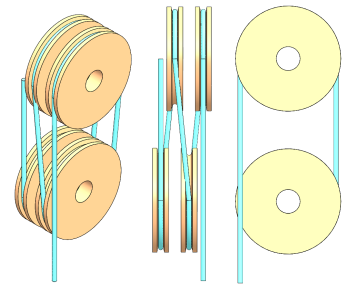
\includegraphics{images/figures/BlockTackleCombined.png}
\end{center}
\caption{To use a single axle, block and tackle ropes cannot sit perfectly
tangential to the pulleys. If this "fleet angle" is small, the system will
still function well.
\label{fig:block_and_tackle}}

\end{figure}

Fleet angle allows our
cable to jog in two dimensions while keeping our pins along the cardinal planes, and this generally makes parts more machinable. Let's add fleet angle
to our cable path. The end result of our design is shown in
Figure~\ref{fig:completed-non-tangential}.

\section{The Plan}

There are multiple ways we could get from our current state (tilted pulleys) to
our desired state (upright but offset pulleys). We'll go about it as
follows (covered in more detail on the following pages):

\begin{enumerate}
\item{} Remove \relation{Tangent} relations on \emph{Line 2}.
\item{} Constrain \emph{Circle 1} \relation{On-Plane} with the \emph{Right Plane}.
\item{} Add a \kode{Plane} \cadsymbol{3d-sketch-plane} to the 3D sketch. We'll make this \relation{On-Plane} with
\emph{Circle 2} in the process of adding it.
\item{} Constrain this \emph{Plane} as \relation{Parallel} to the \emph{Front Plane}.
\item{} Define the distance between the planes to \emph{0.1''}.
\item{} Use construction geometry to constrain \emph{Line 2} in the correct spot.
\end{enumerate}

Our changes will result in Figure~\ref{fig:non-tangential-3d-sketch}.

\begin{figure}[H]
\begin{center}
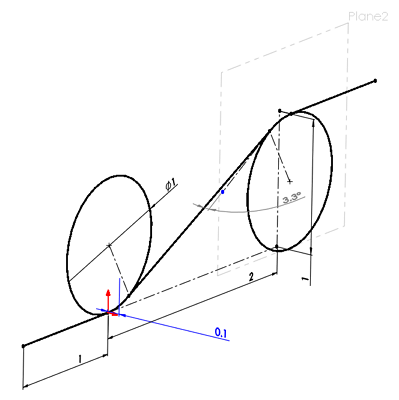
\includegraphics{images/figures/non-tangential-3d-sketch.png}
\end{center}
\caption{Sketch for pulleys with fleet angle.
\label{fig:non-tangential-3d-sketch}}

\end{figure}

\section{Modifying the Sketch}

\label{sec:modify-sketch-fleet-angle}

Start by removing these offending relations in \emph{3D Sketch 1}:

\begin{center}
\begin{tabular}{ccc}
  \hline
  \xrelation{Tangent} & \emph{\sout{Circle 1}} & \emph{\sout{Line 2}} \\
  \xrelation{Tangent} & \emph{\sout{Circle 2}} & \emph{\sout{Line 2}} \\
  \hline
\end{tabular}
\end{center}

Also remove this dimension:

\begin{center}
\begin{tabular}{ccc}
  \hline
  \cadsymbol{dimension} \sout{45\textdegree} & \emph{\sout{Line 1}} & \emph{\sout{Line 2}} \\
  \hline
\end{tabular}
\end{center}

Bring \emph{Circle 1} onto the \emph{Right Plane} with:

\begin{center}
\begin{tabular}{ccc}
  \hline
\relation{On-Plane} & \emph{Circle 1} & \emph{Right Plane} \\
  \hline
\end{tabular}
\end{center}

\begin{aside}
\label{box:overdefine-sketch}
\heading{Over Define or Under Define}

Couldn't we add the relations we want, overdefine the
sketch, and remove the constraints we no longer need, arriving at the same
solution? In theory, yes, but I avoid this because:

\begin{enumerate}
\item{} Overdefined sketches hide which entities are solvable and which aren't.
\item{} Sometimes, SolidWorks struggles to re-solve overdefined sketches, even after
the problem relations are removed.
\item{} The red and yellow lines stress me out, and I much prefer the calming, underdefined
blue lines.
\end{enumerate}
\end{aside}

\section{Planes in 3D Sketches}

Next, add a \kode{Plane} \cadsymbol{3d-sketch-plane} to the sketch,
found amongst the other sketch entities. We'll call this \emph{``Plane 1''}. Select \emph{Circle 2} to
constrain the plane, as in Figure~\ref{fig:add-3d-sketch-plane}. SolidWorks will
infer (correctly) that you want to add a \relation{Coincident} relation between
the plane and \emph{Circle 2}. Note that we do not need to
fully define the plane within the Sketch Plane dialog box.

\begin{figure}[H]
\begin{center}
  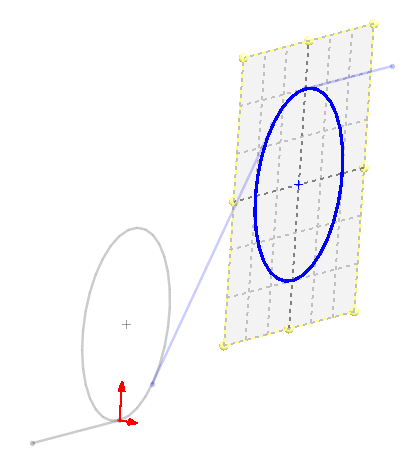
\includegraphics[width=3in]{images/figures/add-3d-sketch-plane.png}
\end{center}
\caption{Add planes within a 3D sketch, a step necessary to constrain the
circles as parallel. \label{fig:add-3d-sketch-plane}}

\end{figure}

We add a plane because planes are easier to manipulate with relations. We cannot make two circles
parallel, but we can make two planes parallel, and draw circles on those planes.
We can also dimension the distance between those two planes. To return to working in the full 3D sketch (rather than on the 2D plane),
double-click in space. Do this now. To reactivate the 2D sketch, which allows you to add
entities coincident with the plane, double-click on the 2-D sketch plane. No
need to do this now.

Both circles are now constrained laterally, but we need the cable (\emph{Line 2}) to run
smoothly between them. Add a construction line as a radius in each circle, as in
Figure~\ref{fig:add-radii}. By making this
radius normal to \emph{Line 2}, we constrain the cable path roughly as it will sit in
real life.

\begin{center}
\begin{tabular}{ccc}
\hline
\relation{Perpendicular} & \emph{Radius 1} & \emph{Line 2} \\
\relation{Perpendicular} & \emph{Radius 2} & \emph{Line 2} \\
\hline
\end{tabular}
\end{center}

\begin{figure}[H]
\begin{center}
  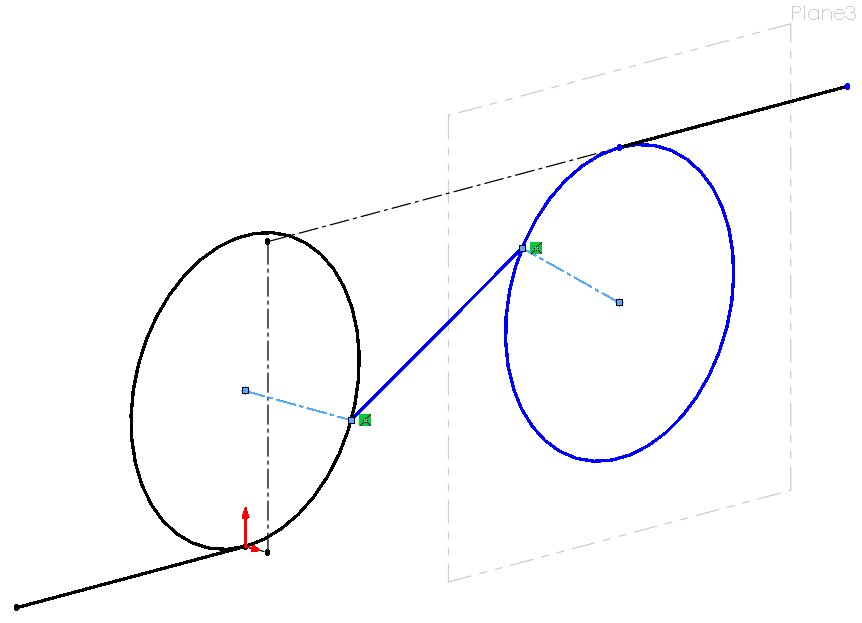
\includegraphics[width=4in]{images/figures/add-radii.png}
\end{center}
\caption{Adding radii to each circle, and making these radii perpendicular to
\emph{Line 2}, places the cable in the correct location. \label{fig:add-radii}}

\end{figure}

Finally, we need to define the distance over which our 0.1'' lateral
departure occurs.  To do this, we need to control the length of the construction
line we added in Section~\ref{sec:cable-rise-run} that is \relation{Along-Z}.
Make this line 2'' long

\begin{figure}[H]
\begin{center}
  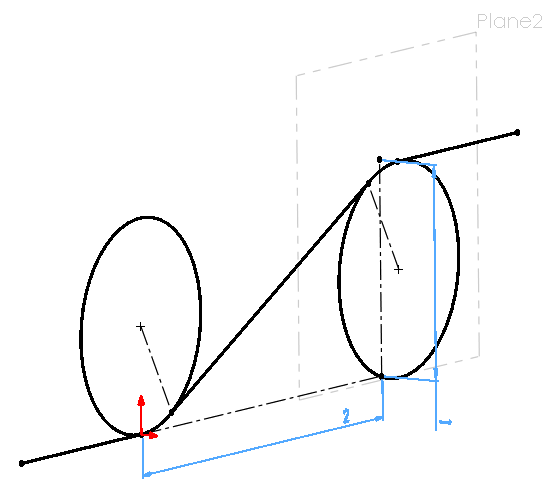
\includegraphics[width=4in]{images/figures/departure-dims.png}
\end{center}
\caption{From Section~\ref{sec:cable-rise-run}, we use three perpendicular lines, one each Along X, Y, and Z, to define the cable
rise and run. Dimension the line Along-Z to 2''. \label{fig:departure-dims}}

\end{figure}

Before we complete our sketch, I like to measure the cable's fleet angle from an ideal,
fully tangential path. To do this, add a \relation{Centerline}
 at where \emph{Line~2} meets \emph{Circle~2}.\footnote{Admittedly, this and most other
 centerlines we used weren't in the center of anything.}Add a
 \relation{Tangent} relation between this centerline and \emph{Circle~2}.
Dimension the angle between this centerline and \emph{Line 2}, as in
Figure~\ref{fig:measure-fleet-angle}. This dimension automatically becomes
``Driven''. My fleet angle measures 3.3\textdegree.

With our sketch fully constrained, we can rebuild \cadsymbol{close-sketch} to arrive
at Figure~\ref{fig:completed-non-tangential}.

\begin{figure}[H]
\begin{center}
  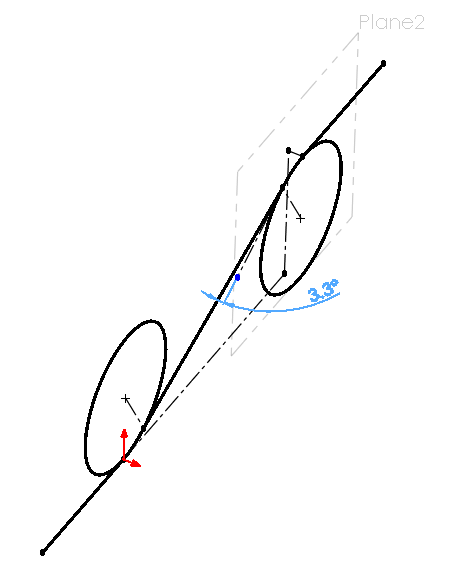
\includegraphics[height=4in]{images/figures/measure-fleet-angle.png}
\end{center}
\caption{Measure the difference between the ideal, tangential path, and the actual
path. \label{fig:measure-fleet-angle}}

\end{figure}

\begin{figure}[H]
\begin{center}
  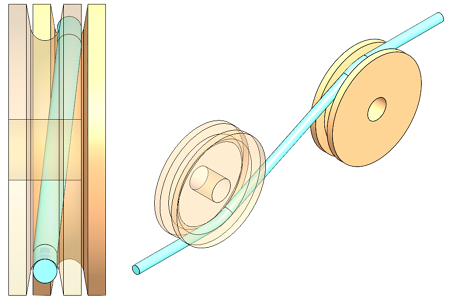
\includegraphics[width=4in]{images/figures/completed-non-tangential.png}
\end{center}
\caption{Completed cable system. While the pulleys remain parallel, the cable jogs
0.1'' laterally. \label{fig:completed-non-tangential}}

\end{figure}

\subsubsection{Section Recap}

\begin{enumerate}
\item{} Remove \relation{Tangent} relations on \emph{Line 2}.
\item{} Constrain \emph{Circle 1} \relation{On-Plane} with the \emph{Right Plane}.
\item{} Add a \kode{Plane} \cadsymbol{3d-sketch-plane} to the 3D sketch. We'll make this \relation{On-Plane} with
\emph{Circle 2} in the process of adding it.
\item{} Constrain this \emph{Plane} as \relation{Parallel} to the \emph{Front Plane}.
\item{} Define the distance between the planes to \emph{0.1''}.
\item{} Use construction geometry to constrain \emph{Line 2} in the correct spot.
\end{enumerate}
